\documentclass[a4paper,norsk,12pt]{article}
\usepackage{amsmath,amssymb,amsthm}
\usepackage{graphicx}
\usepackage[norsk]{babel}
\usepackage[utf8]{inputenc}
\usepackage{float}
\usepackage{bm}
\usepackage{titling}
\usepackage{color}
\usepackage{verbatim}
\usepackage{listings}

\lstset{language=c++}
\lstset{alsolanguage=[90]Fortran}
\lstset{basicstyle=\small}
\lstset{backgroundcolor=\color{white}}
\lstset{frame=single}
\lstset{stringstyle=\ttfamily}
\lstset{keywordstyle=\color{red}\bfseries}
\lstset{commentstyle=\itshape\color{blue}}
\lstset{showspaces=false}
\lstset{showstringspaces=false}
\lstset{showtabs=false}
\lstset{breaklines}

\title{\vspace{-4.0cm} \textbf{Obligatorisk innlevering 1, FYS-MEK1110}}

\author{Av: Laila Andersland, brukernavn:lailaea}



\begin{document}

\maketitle


\subsection*{(a)}

\noindent

Omgivelser: 100m løp 

System: Sprinteren

\begin{figure}[H]
\centering
	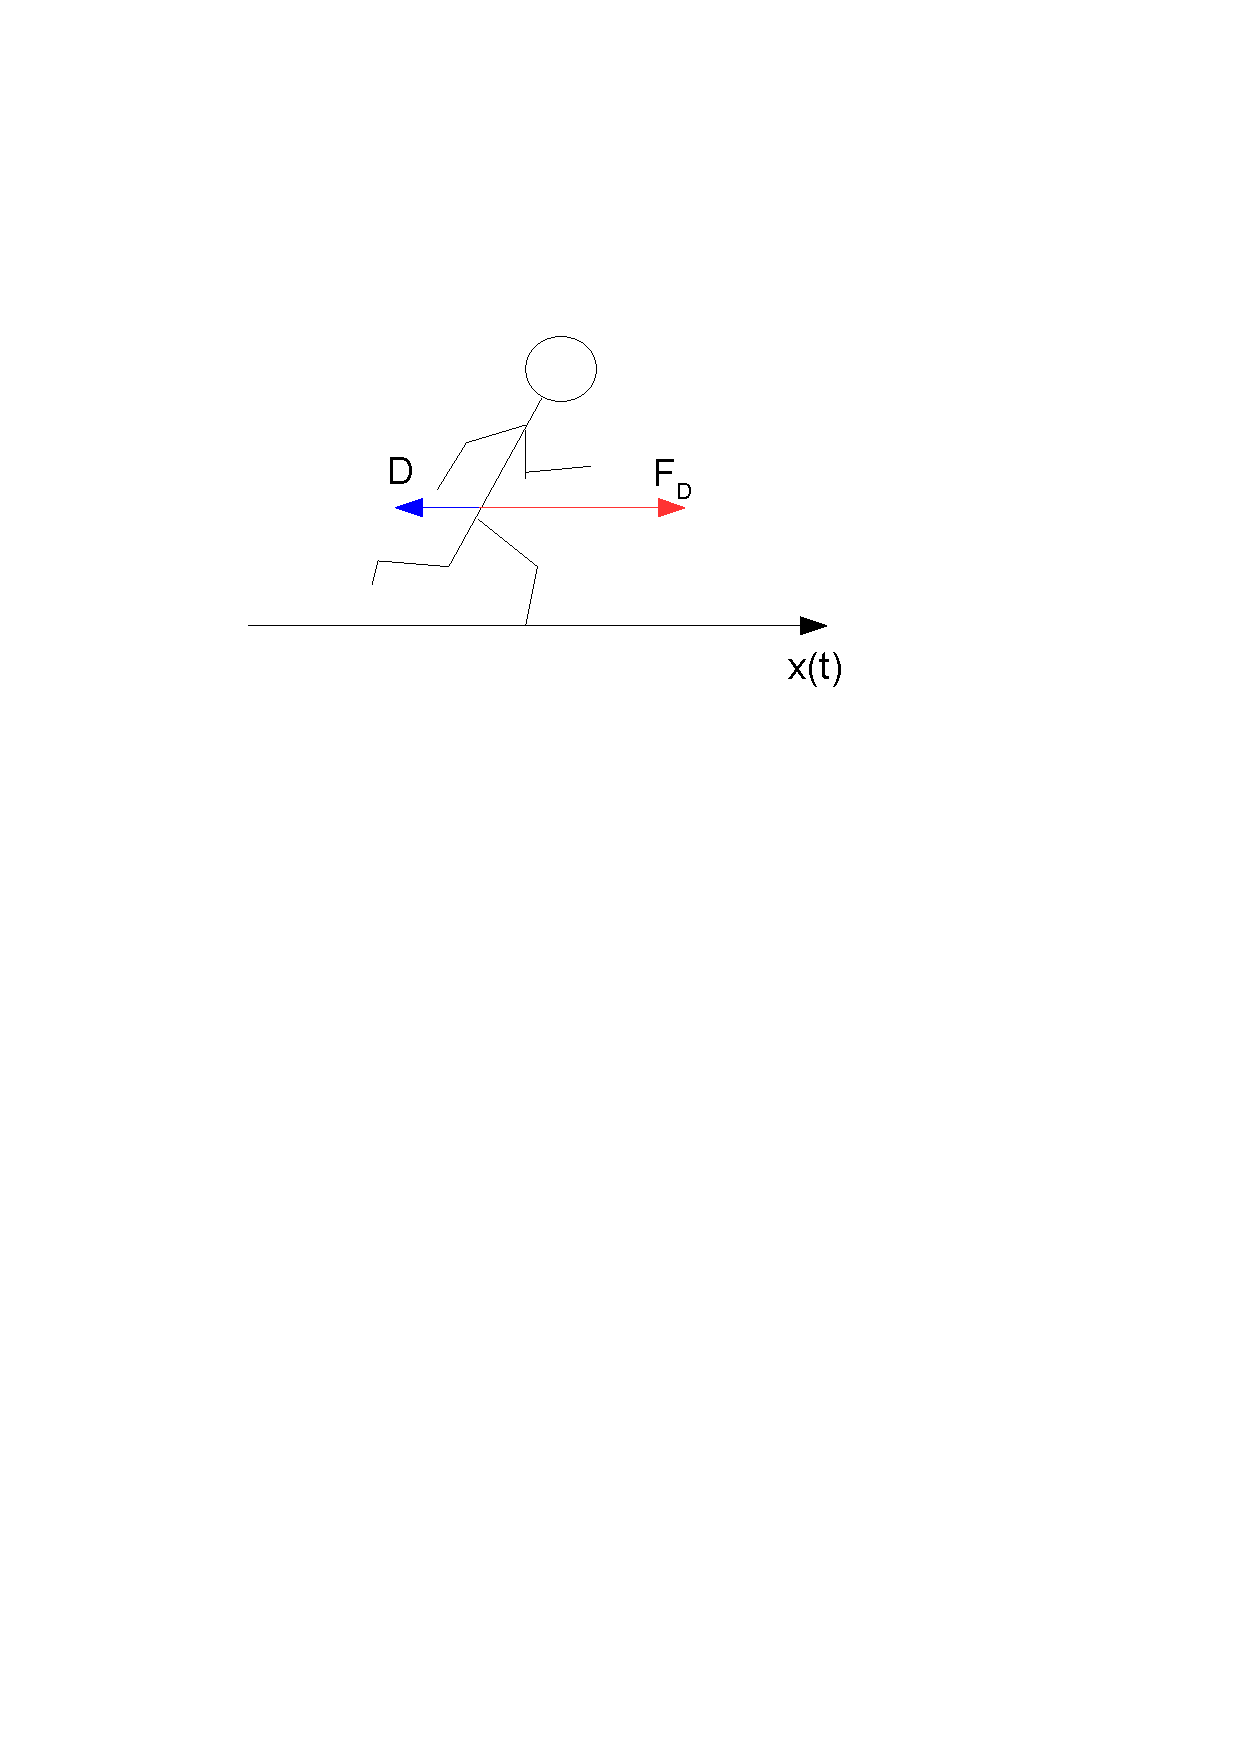
\includegraphics[width=\linewidth, trim={5cm 17cm 5cm 5cm},clip, width=0.5\textwidth,]{sprinter.pdf}
	\caption{Frilegemediagram av sprinteren, med bare horisontale krefter. $F_D$ er drivkraften til sprinteren, og $D$ er luftmotstanden som virker på sprinteren i negativ x-retning. $F_D$ har større kraftpil enn $D$, fordi sprinteren beveger seg i positiv x-retning.}			
	\label{fig:plot1}
\end{figure}

\subsection*{(b)}

\noindent

Vet at akselerasjonen er den tidsderiverte av farten, har derfor at:

$$ v(t) = v_0 + {a_0} \int_0^t dt = v_0 + a_0 t $$

Trekker ut $a_0$ siden den er konstant, og får:

$$ x(t) = x_0 + v_0 t + a_0 \int_0^t \int_0^t dt dt = x_0 + v_0 t + \dfrac{1}{2} a_0 t^2$$


\subsection*{(c)} 

\noindent

Fra Newtons 2'dre lov (N2L):

$$ a = \dfrac{F}{m} = \dfrac{400 kg m/s}{80kg} = 5 m/s^2  $$


Setter inn tiden i uttrykket for posisjonen som vi fant b):

$$ x(6.3s) =  x_0 + v_0 t + \dfrac{1}{2} a_0 t^2 = 0 m + 0 m \cdot 6.3s + 0.5 m/s^2 \cdot 5 \cdot 6.3^2 s^2 = 99.225 \approx 100 m$$


\subsection*{(d)}

\noindent

Vi har luftmotstandsfraft:

\begin{equation}
	D = \dfrac{1}{2} \rho C_D A (v - w)^2
\end{equation}



Her har vi alle størrelsene bortsett fra hastigheten:

$$ D = \dfrac{1}{2} \cdot 1.293 kg/m^3 \cdot 1.2 \cdot 0.45 m^2 (v - 0)^2 = 0.34911 v^2 kg/m $$

Denne kraften virker mot sprinteren når han løper, N2L:

$$ \sum F = F_D - D = ma $$

$$ a = \dfrac{F_D- D}{m}$$

$$ a = \dfrac{400 N - 0.34911 v^2 kg/m}{80 kg} $$

$$ a = 5 m/s^2  - \dfrac{0.34911 v^2 }{80} m/s^2 $$

\newpage
\subsection*{(e)}

Følgende er python koden min:

\lstinputlisting{euler_sprinter.py}

\begin{figure}[H]

  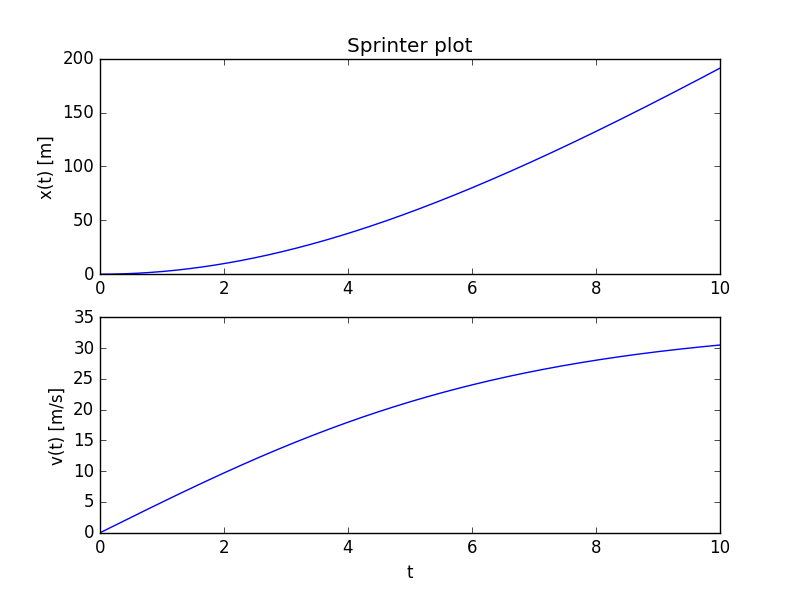
\includegraphics[width=\linewidth]{sprinter01.png}

  \caption{Plot av posisjon x(t) og hastighet v(t) til sprinteren.}

  \label{fig:plot3}

\end{figure}

\noindent
Størrelsen på tidssteg ble valgt til dt=0.01, som er relativt store tidssteg, men siden vi har et lineart uttrykk så vil ikke dette gi noe stort utslag i simuleringen.\\

\noindent
\subsection*{(f)}

\noindent
Utifra Figur 2 ser vi at sprinteren når 100 meteren etter omtrent 6.8 sekunder, som er 0.5 sekunder mer enn hva som ble oppgitt i oppgaven. \\

\noindent
\subsection*{(g)}

\noindent
Vi har en terminalhastighet:

\begin{equation}
	\nu_T = \sqrt{\dfrac{2F}{\rho C_D A}}
\end{equation}

\noindent
Denne oppnåes når farten stagnerer, akselerasjonen er null og drivkraften er like stor som luftmotstanden:

$$ F = D $$


Setter inn for $D$ og $w=0$:

$$ F = \dfrac{1}{2} \rho C_D A v^2 $$


Løser for v:

$$ v^2 = \dfrac{F_D}{(1/2) \rho C_D A} = \dfrac{2 F_D}{ \rho C_D A} $$ 


Som gir utrykket for hastigheten:

$$ v = \sqrt{\dfrac{2 F}{ \rho C_D A}} = \nu_T$$ 


\noindent
Terminalhastigheten er den maksimale hastigheten sprinteren vil oppnå. Gjør en liten modifikasjon på pythonkoden brukt i oppgave e) ved å øke tiden til 30 sekunder:


\lstinputlisting[firstline=20,lastline=22]{euler_sprinter1.py}

\noindent
Som gir følgende plot:

\begin{figure}[H]

  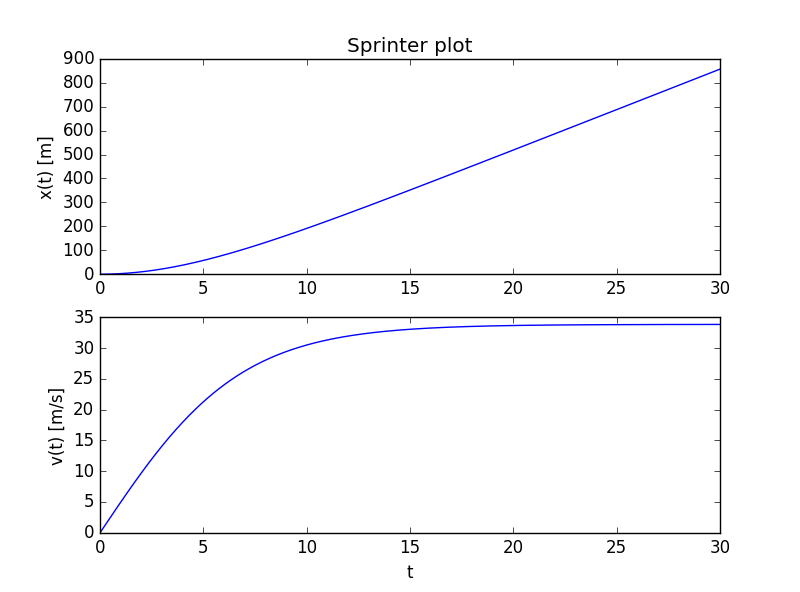
\includegraphics[width=\linewidth]{sprinter02.png}

  \caption{Plot av posisjon x(t) og hastighet v(t) til sprinteren, med økt tid. Her ser man at hastigheten stagnerer etter omtrent 22 sekunder. Den maksimale hastigheten leses av til å være 33 m/s. Dette høres alt for fort ut i forhold til virkeligheten, og det kan være flere grunner til dette. I tillegg til at dette er en simplistisk modell av virkeligheten, så kan en grunn  være at mennesket faktisk ikke klarer å øke farten så lenge uten om å slite seg ut.}

  \label{fig:plot4}
  
\end{figure}

\noindent
\subsection*{(h)}

\noindent
Sprinteren har nå en drivkraft:

$$ F_D = F + F_V = F - f_V v $$

\noindent
$F$ er den konstante kraften og $F_V$ er en negativ kraft som blir større for økende hastighet $v$. Når vi får maksimal hastighet er akselerasjonen null og disse vil være like hverandre:

$$ \sum F = ma $$ 

$$ F - f_V v = 0 $$

$$ F = f_V v $$ 

$$ v = \dfrac{F}{f_V} = \dfrac{400 N}{25.8 sN/m} = 15.5 m/s $$

\noindent
Som begynner å se mer realistisk ut.\\

\noindent
\subsection*{(i)}

En liten oversikt over kreftene:\\

Initial drivkraft:

\begin{equation}
	F_C = f_c exp(-\dfrac{t}{t_c}^2)
\end{equation}


Totale drivkraften:

\begin{equation}
	F_D = F + f_c exp(-\dfrac{t}{t_c}^2) - f_v v
\end{equation}

Luft-motstandskraften med oppdatert areal:

\begin{equation}
	D =\dfrac{1}{2} A (1-0.25 exp(-\dfrac{t}{t_c}^2)) \rho C_D (v-w)^2
\end{equation}

Total kraft på sprinteren blir da:

\begin{equation}
	F_{net} = F + f_c exp(-\dfrac{t}{t_c}^2) - f_v v - D
\end{equation}

\noindent
Implimenterer dette i koden min:

\lstinputlisting{euler_sprinter2.py}

\noindent
Som gir følgende plot:


\begin{figure}[H]

  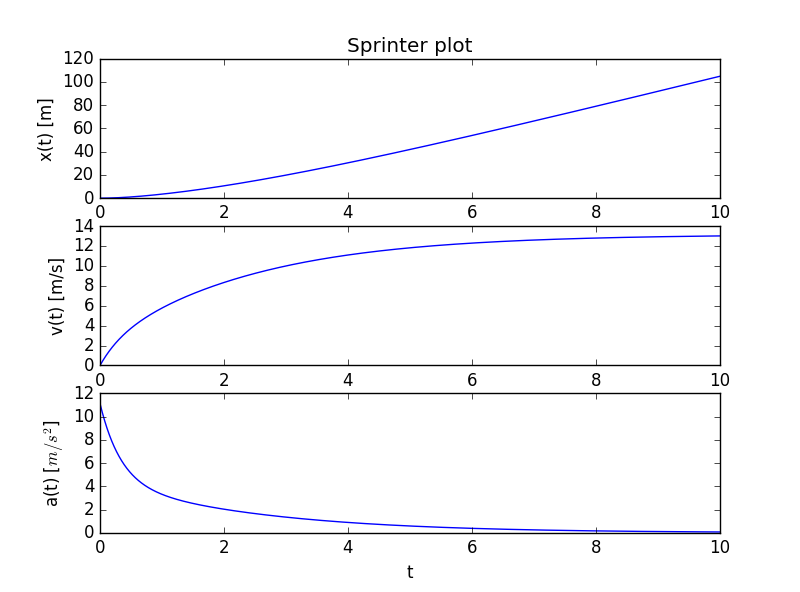
\includegraphics[width=\linewidth]{sprinter03.png}

  \caption{Plot av posisjon x(t), hastighet v(t) og akselerasjon a(t) til sprinteren.}

  \label{fig:plot5}

\end{figure}

\noindent
\subsection*{(j)}

\noindent
Kan lese av plottet at sprinteren når 100meter ved en tid t=9.5 sekunder, altså har den oppdaterte, og litt mer realistiske modellen av systemet gjort at sprinteren løper litt saktere.\\

\noindent
\subsection*{(k)}

\noindent
Utvider koden med en Python-funksjon som returnerer kreftene, og plotter absoluttverdien av disse siden det er mengden vi er interessert i:

\lstinputlisting[firstline=28,lastline=64]{euler_sprinter3.py}

\noindent
som gir følgende plot:

\begin{figure}[H]

  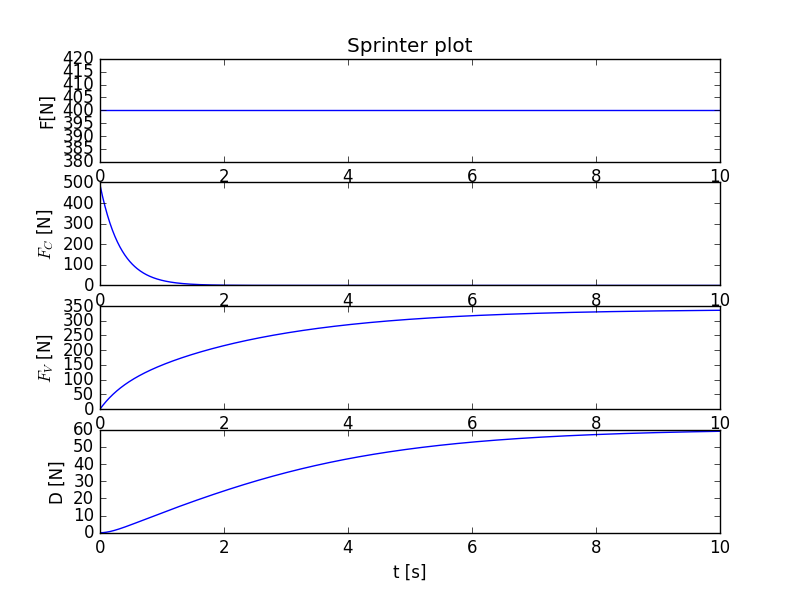
\includegraphics[width=\linewidth]{sprinter04.png}

  \caption{Plot kreftene som virker på sprinteren. }
  \label{fig:plot6}

\end{figure}

\noindent
Når vi ikke tok hensyn til den fysiske begrensningen (med kraften $F_V$) til sprinteren, så løpte sprinteren mye fortere enn hva mennesker kan gjøre. Med initial kraften $F_C$ får vi også simulert denne ekstra kraften i begynnelsen. Ved å bruke alle disse kreftene får vi en mye mer realistisk simulering av et menneske som løper.\\


\noindent
\subsection*{(l)}

\noindent
Oppdaterer programmet:

\lstinputlisting[firstline=25,lastline=25]{euler_sprinter4.py}

\begin{figure}[H]
  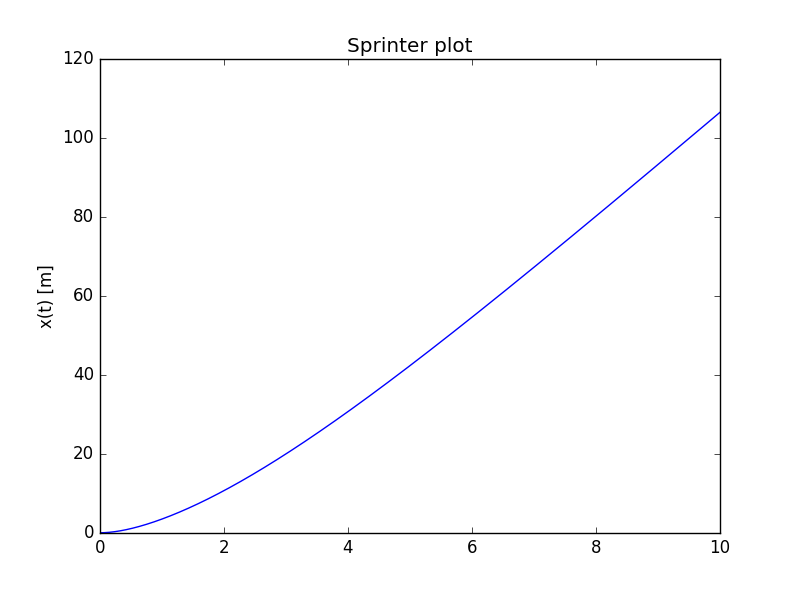
\includegraphics[width=90mm]{sprinter05.png}
  \caption{Plot av posisjonen når $w = 1 m/s$, tiden er 9.5 sekunder.}
  \label{fig:plot7}
\end{figure}

Endrer så retningen på vinden:

\lstinputlisting[firstline=25,lastline=25]{euler_sprinter5.py}

\begin{figure}[H]
  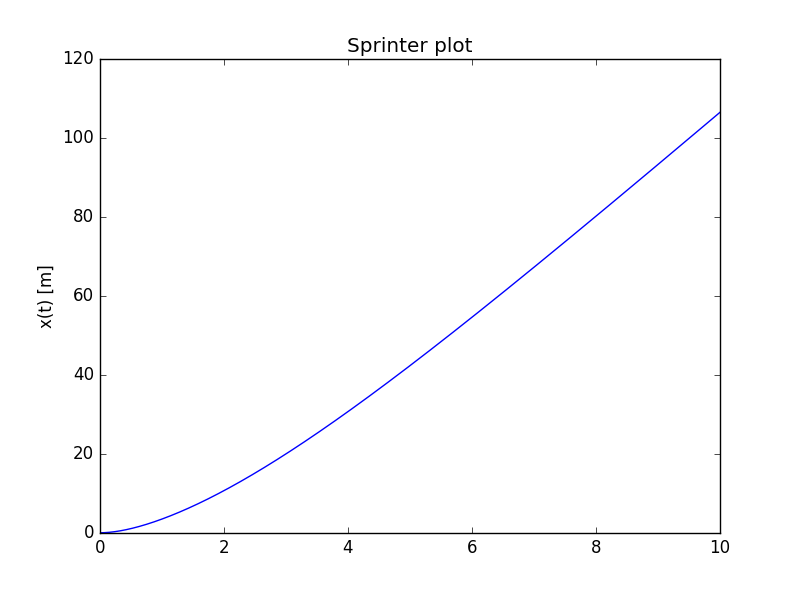
\includegraphics[width=90mm]{sprinter05.png}
  \caption{Plot av posisjonen når $w = -1 m/s$, tiden brukt er 9.71 sekunder }
  \label{fig:plot8}
\end{figure}

\noindent
Det gav altså veldig lite forskjell om sprinter løp med medvind eller motvind på 1 m/s. Kan se utifra utrykket at det vil begynne å gi mye mer effekt for litt større verdier siden den er kvadratisk.

\end{document}
